\documentclass[12pt,letterpaper]{scrartcl}
%\documentclass[12pt,letterpaper]{article}
\usepackage[margin=1in]{geometry}
\usepackage[superscript,biblabel]{cite}
\usepackage{url,graphicx,xcolor,enumitem, array,hyphenat}
\usepackage{hyperref}
\hypersetup{
	colorlinks=true,
	linkcolor=blue,
	filecolor=magenta,      
	urlcolor=cyan,
}

\graphicspath{{figures/}}

%opening
\title{A Tutorial on PCB Design}
\subtitle{--- using KiCad}
\author{Xiaoguang ``Leo'' Liu \\University of California Davis \\ lxgliu@ucdavis.edu}
\date{Aug.~9th, 2015}

\begin{document}

\maketitle

\tableofcontents

\newpage
\section{PCB Basics}

% %\subsection{Example 2: A 2.4\,GHz low noise amplifier (LNA)}

\newpage
\subsection{KiCad}
In the early days, PCBs are designed and laid out literally by hand. See Fig.~\ref{fig:hand-pcb} for an example board from that era. As technologies developed, it become more common to do the job with the help of a computer. Today, there are numerous software tools for PCB design. On the high end, industry-grade packages, such as Cadence Allegro~\footnote{UC Davis students have access to the full suite of Allegro PCB design tools through a donation from Cadence.}, Mentor Graphics Xpedition, and Altium Designer, offer extensive features and capabilities with a high price tag and often a very steep learning curve. On the lower end, popular choices include CadSoft EAGLE, ExpressPCB, and DesignSpark, all of which offer a reasonable set of features at an affordable price. 

\begin{figure}[ht]
\centering
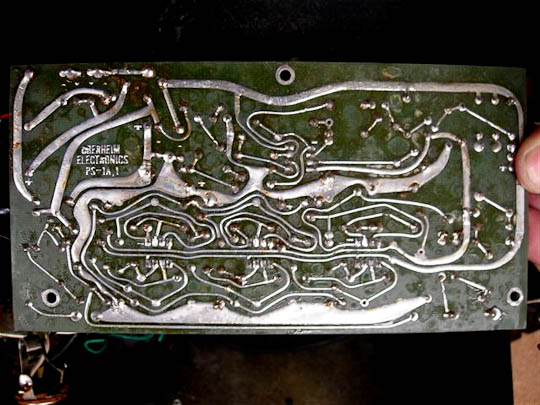
\includegraphics[width=2.5in]{hand-pcb.jpg}
\caption{A vintage PCB laid out by hand~\cite{hand-pcb}.}
\label{fig:hand-pcb}
\end{figure}

In recent years, KiCad has emerged as a popular open-source software package for designing and laying out PCBs~\cite{kicad}. KiCad is available on all three major personal computer operating systems, Windows, Linux, and Mac OS. 
Compared with the above mentioned software packages, KiCad is completely free of charge or any other limitation. Although KiCad is not as sophisticated as industry-level tools, it is capable of dealing with fairly complicated designs, and the active developer community is working hard to improve its capabilities. In fact, as of this writing, KiCad has not had an official stable release for the last two years because of the constant development progress being made. In this tutorial, we will using a recent build \#6055, dated Aug.~8th, 2015.

Fig.~\ref{fig:kicad-main} shows the main window of KiCad. The main window serves as a project management panel where you can launch the individual PCB tools. 

\begin{figure}[ht]
\centering
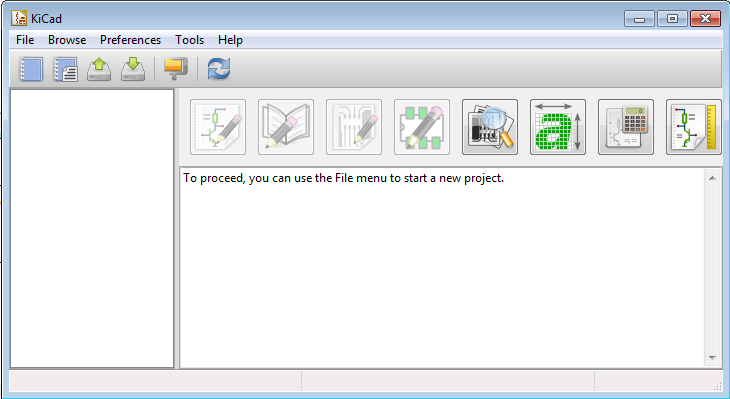
\includegraphics[width=5in]{kicad-main.png}
\caption{The main window of KiCad.}
\label{fig:kicad-main}
\end{figure}

\begin{table}[ht]
\caption{Individual tools within KiCad.}
\begin{tabular}{|m{0.5in}|m{2.5in}||m{0.5in}|m{2.5in}|}
\hline 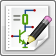
\includegraphics[width=0.5in]{eeschema-icon}  &   Eeschema: schematic editor/capture tool & 
\includegraphics[width=0.5in]{gerbview-icon} &  Gerbview: Gerber file viewer\\ 

\hline 
\includegraphics[width=0.5in]{sche-lib-icon} &  Schematic symbol editor & 
\includegraphics[width=0.5in]{bitmap2component-icon} &  Bitmap2Component: A tool for creating component symbol from a picture\\ 

\hline 
\includegraphics[width=0.5in]{pcbnew-icon} &  Pcbnew: PCB layout tool & 
\includegraphics[width=0.5in]{calculator-icon} &  A calculator for common PCB design related calculations\\ 

\hline 
\includegraphics[width=0.5in]{footprint-lib-icon} &  Component footprint editor & 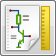
\includegraphics[width=0.5in]{pi-editor-icon} &  Schematic sheet layout editor\\ 
\hline 
\end{tabular} 
\end{table}

\newpage
\section{Example 1: Arduino dice}
In the first example we will make a small eletronic dice consisting of a ATmega328P microcontroller\footnote{The heart of the Arduino UNO platform.}, a switch, a 7-segment LED display, and some misc resistors and capacitors. Every time you press and release the switch, the microcontroller will generate a random number (1--6) for the dice value and display it on the 7-segment LED. This example is a stripped down version of a project from PrinceTronics~\cite{dice}. 

Table.~\ref{tab:example1} lists the components that are needed for this example.

\begin{table}[h]
\centering
\caption{List of components for Example 1.}
\begin{tabular}{|c|c|c|}
\hline \bf  Item Description & \bf Quantity & \bf Digikey Part \# \\ 
\hline \hline  Arduino Uno board, DIP version & 1 & \href{http://www.digikey.com/product-detail/en/A000066/1050-1024-ND/2784006}{1050-1024-ND} \\ 
\hline  16-MHz crystal oscillator &  1 & \href{http://www.digikey.com/product-search/en?KeyWords=300-8499-ND}{300-6034-ND} \\ 
\hline  22-pF ceramic capacitor, SMD, 0603, 5\% & 2 & \href{http://www.digikey.com/product-detail/en/C1608C0G1H220J080AA/445-1273-1-ND/567670}{445-1273-1-ND}  \\ 
\hline  1-uF ceramic capacitor, SMD, 0603 & 1 & \href{http://www.digikey.com/product-detail/en/CL10F105ZP8NNNC/1276-1041-1-ND/3889127}{1276-1041-1-ND}  \\ 
\hline  10k-Ohm resistor, SMD, 0603, 1/10W, 5\% & 2 & \href{http://www.digikey.com/product-detail/en/ERJ-3GEYJ103V/P10KGCT-ND/134717}{P10KGCT-ND} \\ 
\hline  Push button switch, 0.05 A, 24 V  & 1 & \href{http://www.digikey.com/product-search/en?KeyWords=SW400-ND}{SW400-ND} \\ 
\hline  7-segment 1-digit display, 
common cathode & 1 & \href{http://www.digikey.com/product-detail/en/HDSP-313E/516-2734-ND/2219051}{516-2734-ND} \\ 
\hline 
\end{tabular} 
\label{tab:example1}
\end{table}

\subsection{Schematic Capture}

\begin{enumerate}
	\item Click on the Eeschema icon. A new schematic window should appear.
	\item Save your schematic design with the file name ``arduino\_dice.sch''. 
	\item The default library that comes with KiCad installation has schematic symbols for many ATmel micro-controllers, including the ATmega328P that is used on the Arduino platform. You can place the symbol on your schematic by the following steps. 
		\begin{enumerate}
			\item Click on the ``Place a component'' button from the toolbar on the right side.
			
				\begin{figure}[h]
					\centering
					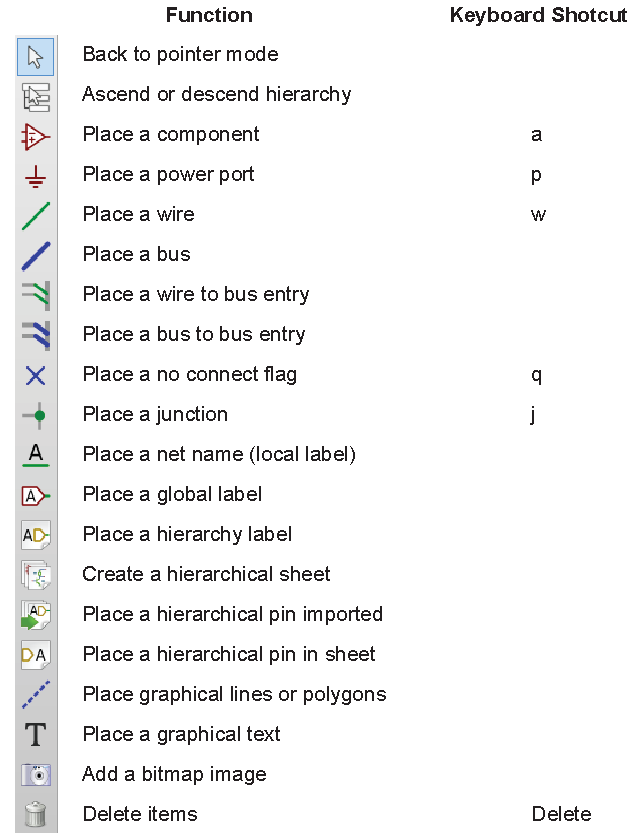
\includegraphics{eeschema-toolbar}
					\caption{Eeschema toolbar icons.}
					\label{fig:eeschema-toolbar}
				\end{figure}
				
			\item Click anywhere on the schematic, a dialog box should appear. 
				\begin{figure}[h]
					\centering
					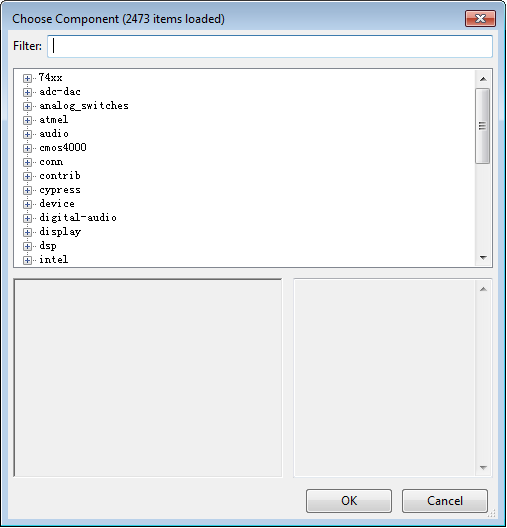
\includegraphics[width=3in]{place-component.png}
					\caption{Place component dialog box.}
					\label{fig:place-component}
				\end{figure}

			\item We'll add our first item, the ATmega328P microcontroller, from the ``atmel'' library. Select the ``atmel'' entry, and click ``OK''. A new dialog box appears for you select the particular device, the “ATMEGA328P-P”. Click ``OK''. Note that if you already know the name of the component, you can simply start typing the name and Eeschema will filter out the components with the same initial characters. It wouldn't take long before you arrive at your desired component.
			
			\item The ATmega328P symbol should now cling to your mouse cursor. Click on the schematic to place it at a location you like. 
			\item A number of component editing operations are available by right clicking on the component. Some of the operations have keyboard shortcut. The general way to use the shortcut is to place the cursor on the component and press the corresponding shortcut key. Pressing the ``ESC'' key will cancel the current operation. 
			
			\begin{figure}[h]
				\centering
				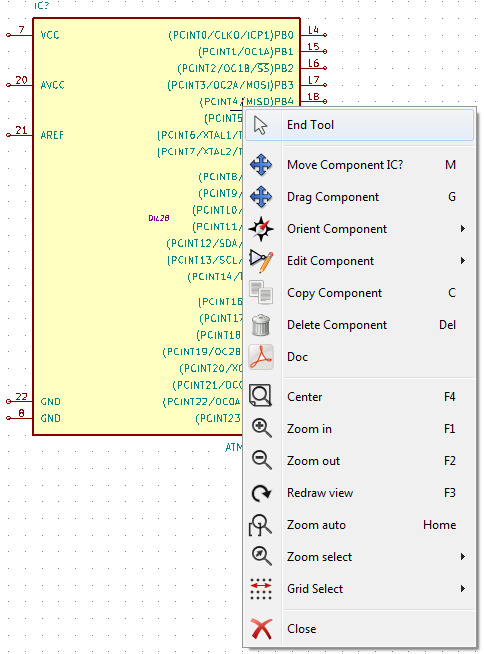
\includegraphics[width=3in]{edit-component}
				\caption{Edit component pop-up menu.}
				\label{fig:edit-component}
			\end{figure}

				\begin{enumerate}
					\item ``Move component'' will move the component and break all circuit connections to it. To retain the connections, use ``Drag component''. 
					\item ``Orient component'' has further options to rotate and mirror the component. Experiment the shortcuts by pressing ``r'' or ``y'' while placing the cursor on the component.
					\item ``Edit component$\rightarrow$ Edit'' will bring up a dialog box that allows you to edit all of the component properties. 
						\begin{enumerate}
							\item The ``Reference'' and ``Value'' are the two properties that you are most likely to edit in this dialog box. ``Reference'' is the annotation of the component. In this case, it should read ``IC1''. You may also write it as ``IC?'' where the ``?'' is a placeholder for a numeric value. KiCad can auto annotate the components and assign a unique value for each component; we will look at how to do this shortly.
							\item The ``Value'' entry is usually used to mark the component value. For resistors, capacitors, and inductors for examples, the ``Value'' can simply be their corresponding resistance, capacitance, and inductance values. For this ATmega microcontroller we will simply use the ``Value'' to mark the component’s name. 
							\item For now, we will delete the value for the ``Footprint'' field. 
						\end{enumerate}
				\end{enumerate}
		\end{enumerate}

	\item Follow a similar procedure to place the other circuit components. Table.~\ref{tab:example1-sche} lists which library they belong to and their names in the library. 
	
	Note that the \emph{Vcc} and \emph{ground} symbols, and all other symbols related to providing power to the circuits, are organized into the \emph{power} library. They can be accessed directly by clicking the \emph{Place a power port} button from the toolbar on the right. Place a \emph{Vcc} and several \emph{GND} pins where necessary.
	
		\begin{table}[ht]
			\centering
			\caption{Schematic components for Example 1.}
			\begin{tabular}{|c|c|c|c|}
			\hline \bf Component & \bf Library & \bf Name in Library & \bf Value \\
			\hline 
			\hline ATmega328P & atmel & ATMEGA328P-P & \\
			\hline Two 22-pF capacitors & device & C & 22\,pF \\ 
			\hline One 1-uF capacitor & device & C & 1\,uF \\ 
			\hline One 16-MHz crystal oscillator & device & CRYSTAL & 16\,MHz \\ 
			\hline One 7-segment LED display & display & 7SEGMENTS &  \\ 
			\hline One push button & device & SW\_PUSH &  \\ 
			\hline Two 10-k resistors & device & R & 10\,k \\ 
			\hline 2-pin header &  conn & CONN\_01X02 &  \\ 
			\hline Vcc & power & vcc &  \\ 
			\hline Ground & power & GND &  \\ 
			\hline 
			\end{tabular}
			\label{tab:example1-sche}
		\end{table}
	\item Connect the components together according to Fig.~\ref{fig:example1-schematic-1} by placing wires between corresponding pins. The components should be arranged to make connecting them together easier with less wire clutter. To start placing a wire, click on the ``Place a wire'' button, then click on the starting point, and finish by clicking on the endpoint of the wire. It is often easier to use the keyboard shortcut. First move your cursor to the starting point and press the ``w'' key. A wire is started at the cursor location. Move the cursor to the endpoint and click to finish the connection. 
	
		\begin{figure}[h]
			\centering
			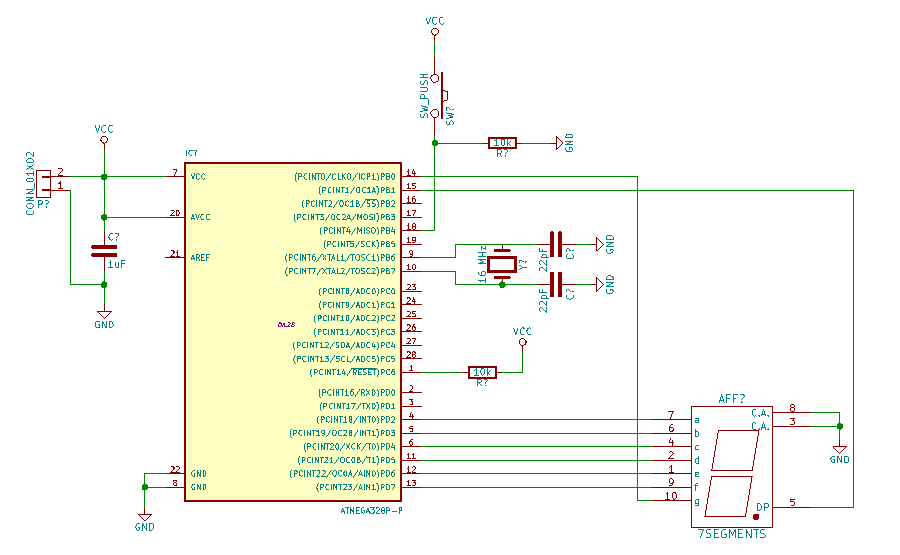
\includegraphics{example1-schematic-1}
			\caption{Initial schematic drawing of Example 1 circuit.}
			\label{fig:example1-schematic-1}
		\end{figure}
	
	\item The schematic drawing can become difficult to read if there are too many wire crossovers. ``Named netlist'' can be used to alleviate the issue. Although our example circuit is quite simple and easy to read, we will still use it to illustrate how to ``clean up'' the schematic with named net.
		\begin{enumerate}
			\item Delete the wire between the ATmega328P's \emph{PB1} pin and the 7-segment LED's \emph{DP} pin. 
			\item Draw a short section of wire on the ATmega328P's \emph{PB1} pin; one of the ends of the wire is now floating. 
			\item Click the ``Place a net name -- local label'' button and then click on the schematic. A dialog box will appear, input ``DP'' in the ``Text'' field, and click ``OK''. The text ``DP'' can now be seen to cling on the cursor. 
			\item Click on the floating terminal of the short wire on the \emph{PB1} pin to finish naming a net. You should now see the text DP attached to the wire on the \emph{PB1} pin; the little hollow square at the floating end of the wire has also disappeared. 
			\item Repeat steps b--d for the \emph{DP} pin of the 7-segment LED. The ATmega328P's \emph{PB1} pin and the 7-segment LED's \emph{DP} pin are now connected by the net name ``DP'' even though there is no direct wire connection on the schematic view. 
			\item Repeat steps a--e for the connection between ATmega328P's \emph{PB4} pin and the push button. Refer to the final schematic (Fig.~\ref{fig:example1-schematic-final}) for how it looks.  
		\end{enumerate}
	
	\item In most circuits, the unused pins can be left floating. In this example, however, we will terminate all the unused pins by placing a no connect label on them; this tells KiCad to ignore these pins during the electrical rule check (ERC).
	
	\item The schematic capture is now almost done. Notice that the references to some of the components still have question marks. For example, the two capacitors connected to the crystal oscillator look identical to each other; we need to differentiate them. In KiCad, we do this by annotating the schematic, i.e. giving each component a unique identifier (reference). Annotation can be done manually by changing the ``Reference'' property of a component and making sure that each reference is unique, but it is much easier to let KiCad do the annotation automatically. 
		\begin{enumerate}
			\item Click the ``Annotate'' button. 
			\item A dialog box appears. The options are all self-explanatory. 
		
			\item Click the ``Annotate'' button to finish. You must have noticed that you can ``un-annotate'' the schematic by clicking the ``Clear annotation'' button. 
			
			\item After annotation, you should see that all the components are numbered. 
		\end{enumerate}
		
	\item It is always a good idea to run an ERC before proceeding. ERC checks the electrical connections between components and try to detect potential errors in the schematic.
	
	\item Once you’ve passed the ERC, generate a netlist by clicking the ``Generate netlist'' button.
	
	\item This will create a netlist file that describes the circuit connections. The netlist file will be used to guide the PCB layout process.
	
	\item The final schematic should look like that in Fig.~\ref{fig:example1-schematic-final}.
		\begin{figure}[h]
			\centering
			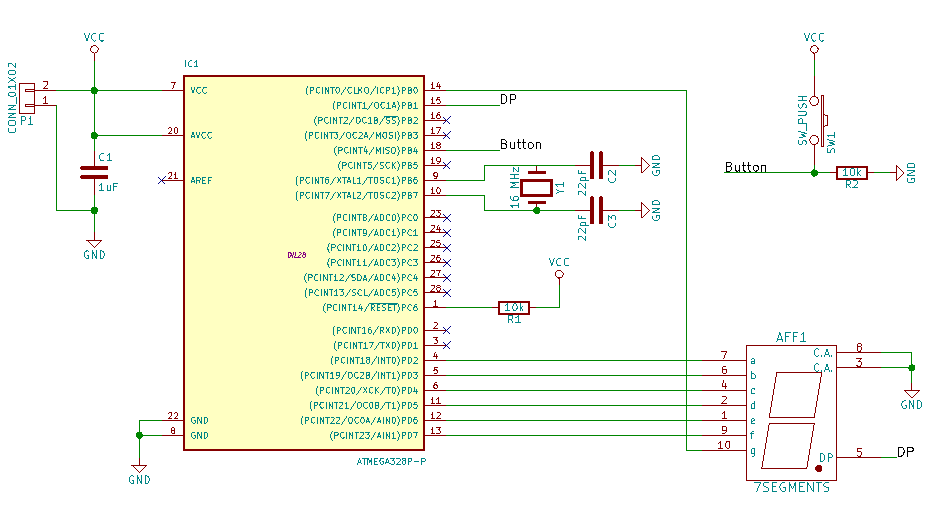
\includegraphics{example1-schematic-final}
			\caption{Completed schematic drawing of Example 1 circuit.}
			\label{fig:example1-schematic-final}
		\end{figure}		
\end{enumerate}

%\newpage
%\subsection{Creating or Editing Schematic Symbols}
%Sometimes you run into a situation where you can’t find a proper symbol in the default KiCad library for the component that you want to use. The following steps will show you how to create a schematic symbol of your own. 
%
%\begin{enumerate}
%	\item From the KiCad project window, click the ``Schematic library editor'' button 
\includegraphics[width=0.3in]{sche-lib-icon} to launch the schematic symbol editor and library manager. Alternatively, you can launch it by clicking the same button from Eeschema. The library editor window should appear.
%	
%	\begin{figure}[h]
%		\centering
%		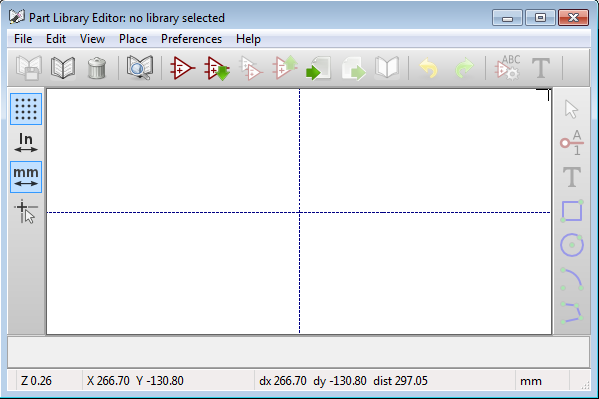
\includegraphics[width=0.6\linewidth]{sche-lib-editor}
%		\caption{The schematic library editor program}
%		\label{fig:sche-lib-editor}
%	\end{figure}
%	
%	\item Click the ``Select working library'' button to set the current working library. A dialog box should appear with the same list of component libraries that we saw when we placed components on the schematic. 
%		\begin{enumerate}
%			\item If you are creating a new component, it is recommended that you select the project library, which is by default named ``\textit{project\_name}-cache'' and should be the last one in the list. In this example, select the library named ``arduino\_dice-cache''. 
%			
%			\item If you are trying to edit an existing component, click the corresponding library.
%			
%			\item Click ``OK'' to finalize the selection. 
%		\end{enumerate}
%	
%	\item In this example, we are actually not missing any schematic symbol. Just for the sake of demonstrating how to use the library editor, we will build our own version of the ATmega328P microcontroller IC. Fig. shows the pin diagram of the ATmega328P~\cite{atmega328p}.
%		\begin{figure}[h]
%			\centering
%			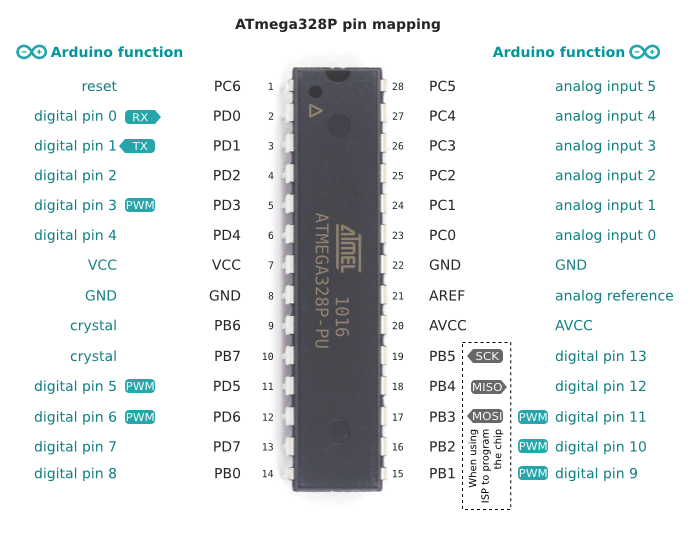
\includegraphics[width=5in]{atmega328p-pins}
%			\caption{Pin mapping for the ATmega328P microcontroller.}
%			\label{fig:atmega328p-pins}
%		\end{figure}
%
%	\item Click the ``Create a new component'' button. A dialog box will appear. Put \nohyphens{``ATmega328p''} as the component name. Leave everything else as default. Worth mentioning is the ``Number of parts per package'' setting. Sometimes a component may have many pins and it becomes difficult to route the schematic (or to be more precise, it becomes difficult to read the schematic when you have lots of wire connections). It may be easier to split a component into several schematic symbols so that routing can be easier. In such a scenario, you can have multiple parts per package. 
%		\begin{figure}[h]
%			\centering
%			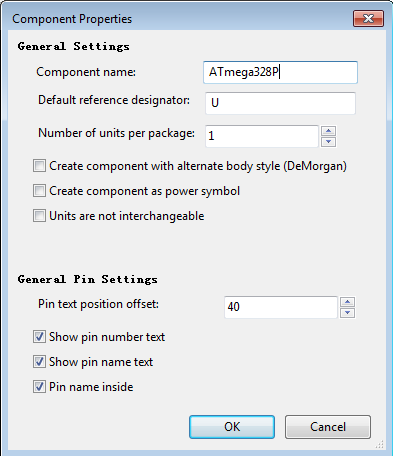
\includegraphics[width=3in]{create-component}
%			\caption{Creat component dialog box.}
%			\label{fig:create-component}
%		\end{figure}
%		
%	\item Click ``OK'' and you should see the component ``Reference'' and ``Value'' strings appearing near the center of the library editor main window. 
%	
%	\item Click the ``Add graphic rectangle to the component body'' button , and use the mouse cursor to draw a rectangle from $(x=-0.400'', y=0.700'')$ to $(0.400'',-0.700'')$ (Fig.~\ref{fig:draw-rectangle-symbol}). The current position of the cursor is displayed at the bottom of the main window. Notice that the positive direction of the $y-$axis points downward. 
%		\begin{figure}[h]
%			\centering
%			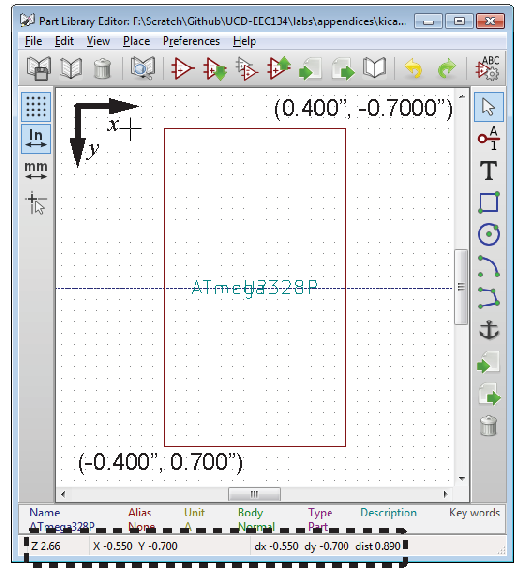
\includegraphics{draw-rectangle-symbol.pdf}
%			\caption{Drawing a rectangle in the library editor main window with the help of the built-in cordinate system.}
%			\label{fig:draw-rectangle-symbol}
%		\end{figure}
%		
%	\item Add component pins. 
%		\begin{enumerate}
%			\item Click the ``Add pins to the component'' button 
%			
%			\item Click anywhere in the main drawing window. A dialog box should appear. Put ``PC6'' for the ``Pin name'', ``1'' for the ``Pin number'', ``Right'' for the ``Orientation'', ``Input'' for the ``Electrical type'', and leave everything else as default. 
%			
%			\item Click ``OK'', and then click at $(-0.600, -0.650)$ to add the pin. 
%		\end{enumerate}
%
%	\item Repeat the above process and add the rest of the pins as follows. 
%		\begin{table}[h]
%			\centering
%			\begin{tabular}{|p{0.5in}|p{0.5in}|p{0.5in}|p{1in}||p{0.5in}|p{0.5in}|p{0.5in}|p{1in}|}
%				\hline  \bf Pin Name & \bf Pin number & \bf Orien- tation & \bf Electrical Type & \bf Pin Name & \bf Pin number & \bf Orien- tation & \bf Electrical Type\\ 
%				\hline \hline PD0 & 2 & Right & Input & PC5 & 28 & Left & Input\\ 
%				\hline PD1 & 3 & Right & Input & PC4 & 27 & Left & Input\\ 
%				\hline PD2 & 4 & Right & Input & PC3 & 26 & Left & Input \\ 
%				\hline PD3 & 5 & Right & Input & PC2 & 25 & Left & Input\\ 
%				\hline PD4 & 6 & Right & Input & PC1 & 24 & Left & Input\\ 
%				\hline VCC & 7 & Right & Power Input & PC0 & 23 & Left & Input\\ 
%				\hline GND & 8 & Right & Power Input & GND & 22 & Left & Power Input\\ 
%				\hline PB6 & 9 & Right & Input & AREF & 21 & Left & Input\\ 
%				\hline PB7 & 10 & Right & Input & AVCC & 20 & Left & Power Input\\ 
%				\hline PD5 & 11 & Right & Input & PB5 & 19 & Left & Input\\ 
%				\hline PD6 & 12 & Right & Input & PB4 & 18 & Left & Input\\ 
%				\hline PD7 & 13 & Right & Input & PB3 & 17 & Left & Input\\ 
%				\hline PB0 & 14 & Right & Input & PB2 & 16 & Left & Input\\ 
%				\hline & & & & PB1 & 15 & Left & Input\\
%				\hline 
%			\end{tabular} 
%		\end{table}
%	
%	\item Now move the ``Reference'' string above the rectangle (only for aesthetic reasons) and the ``Value'' string below the rectangle. You can also add a half circle (arc) to the top of the rectangle to indicate the orientation of the component. The completed component looks that in. 
%		\begin{figure}[h]
%			\centering
%			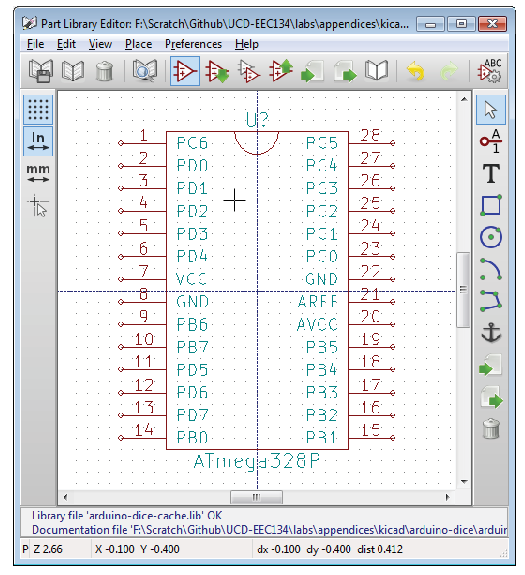
\includegraphics{draw-rectangle-symbol-final.pdf}
%			\caption{Completed schematic symbol for the ATmega328P microcontroller.}
%			\label{fig:draw-rectangle-symbol-final}
%		\end{figure}
%		
%	\item Click the “Save current library to disk” to save your work. This should complete the creation of the schematic symbol. To verify that you have successfully created the symbol, go back to the Eeschema window and check whether you can find the ATmega328P symbol you just built in the ``arduino-dice-cache'' library. 
%	
%\end{enumerate}

\subsection{Associating schematic symbols with footprint}
In KiCad, the schematic symbol and the footprint of a device are stored in separate files (.lib for schematic symbols and .mod for footprint). In order for the PCB layout tool (Pcbnew) to put the correct footprints in the layout, we need to assign a relationship between the schematic symbols and the footprints in a circuit. The program CvPcb is used to do this. 

\begin{enumerate}
	\item Open CvPcb from the Eeschema window. By default, CvPcb should automatically loaded the netlist of the project. If not, you can go to “File->Open” to open the desired netlist. Ignore any error messages at this stage.
	
	\item The CvPcb window consists of three panes. The leftmost one lists the footprint libraries. The center one lists all the schematic components used in the circuit. The right one presents a list of available footprints. These footprints are installed with the KiCad program. By default, CvPcb presents only footprints that it thinks that are relevant to the components. To see a full list of available components, uncheck the ``Filter footprint list by keywords'' button. 
	
	\item Our job in CvPcb is to associate the schematic components with their corresponding footprint. This is done by first selecting the component in the left pane, and then double clicking on the right footprint in the right pane. You can preview the drawing of the footprint by clicking the ``View selected footprint'' button . 
	
	\item \textbf{A very important rule in PCB design is to never trust footprints provided by others unless 1) they are directly from the component vendors; 2) you have verified them yourself.} The default footprint library that comes KiCad is particularly error prone. For this reason, we will be creating all the footprints by ourselves in this example. The next section outlines this process. 
\end{enumerate}

\subsection{Creating or Editing Footprint}

\subsubsection{SMD Capacitor}

We will start with the simplest component in the circuit, the 22\,pF capacitor. This capacitor is a 0603 SMD capacitor produced by TDK Corporation. ``0603'' refers to its lateral dimensions in thousandth of an inch (normally referred to as a \textbf{mil} or a \textbf{thou}), that is, the capacitor is roughly 60\,mil long and 30\,mil wide. If we look at the dimension drawing provided by the vendor (Fig.~\ref{fig:tdk_cap_datasheet}a), we see that its actual dimensions are 63\,mil$\times$31\,mil. In fact, the capacitor is realy sized in the metric system, with a nominal dimension of 1.6\,mm$\times$0.8\,mm. So this capacitor is a ``0603'' in imperial units and ``1608'' in metric units. \textbf{The difference between the imperial and metric units is a common source of confusion when choosing components. Alwasy double check!}

On the \href{http://www.digikey.com/product-detail/en/C1608C0G1H220J080AA/445-1273-1-ND/567670}{Digikey product page}, we can find the datasheet to the capacitor \href{http://product.tdk.com/en/catalog/spec/mlccspec_commercial_general_midvoltage_en.pdf}{``C Series, Gen Appl \& Mid-Voltage Spec''}. Page 15 of the datasheet, copied here in Fig.~\ref{fig:tdk_cap_datasheet}b, shows the recommended land pattern (footprint) for the capacitors in this serie of products. The recommended dimensions for the 0603 (1608) capacitor is highlighted; here we will use the median value of 0.7\,mm for A, B, and C. 

	\begin{figure}[ht]
		\centering
		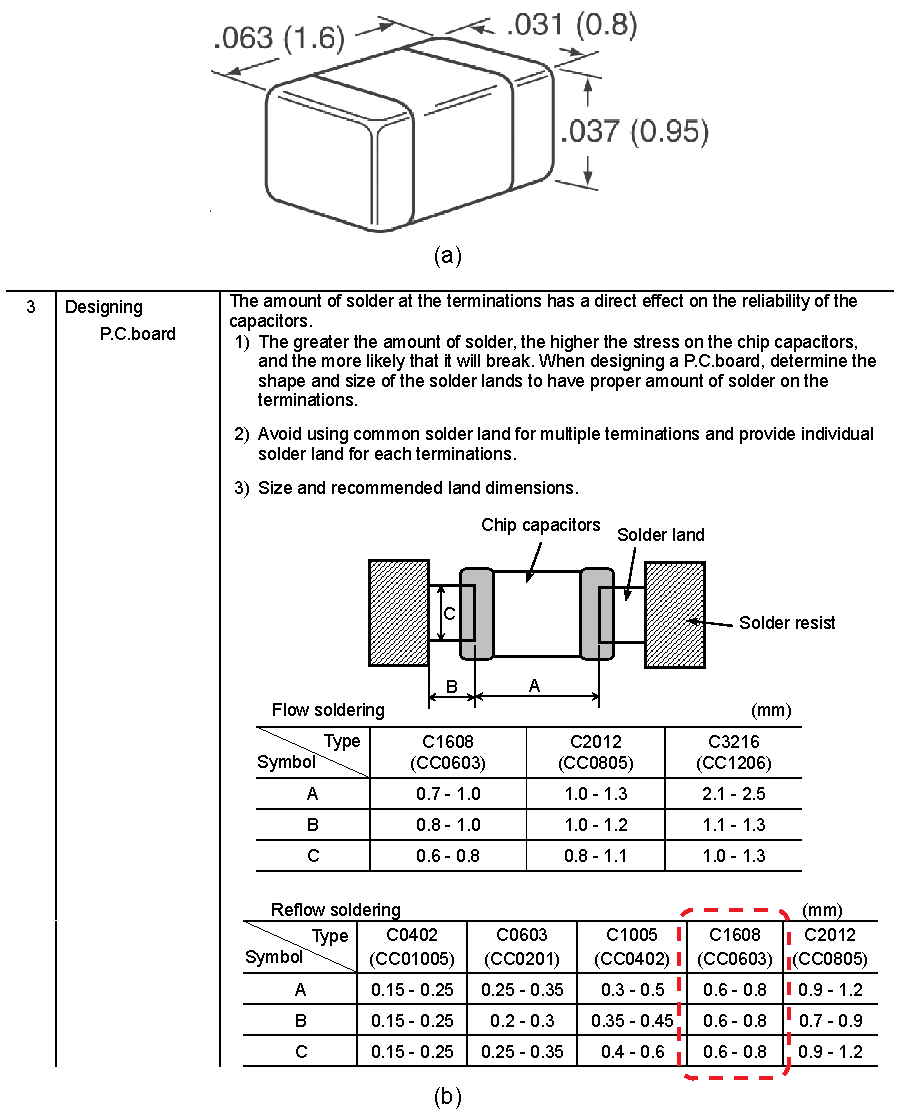
\includegraphics{tdk_cap_datasheet}
		\caption{(a) Dimensions of the TDK C-series 22\,pF SMD capacitors. (b) PCB design recommendation for TDK C-series SMD capacitors. Land pattern dimensions for the C1608 type is highlighted in red.}
		\label{fig:tdk_cap_datasheet}
	\end{figure}

Now let's start drawing the footprint for the capacitor. 
\begin{enumerate}
	\item Start the PCB footprint editor by clicking on the ``PCB footprint editor'' button. 
	
	\item Click the ``New footprint'' button to create a new footprint. Put ``smd\_0603'' as the name in the pop-up dialog box. Click ``OK''. 
	
	\item By default, the footprint name ``smd\_0603'' and the Reference string ``REF**'' will appear in the center of the drawing window. 
	
	\item Set the working unit to ``mm'' (millimeters). Then set the grid size to ``User grid''. The user grid size can then by set by going to menu ``Dimensions$\rightarrow$ User Grid Size''. Set the unit to ``Millimeters'', ``Size X'' to ``0.05'', and ``Size Y'' to ``0.05''.
	
	\item Click the ``Add pads'' button. Move the cursor to position (-0.7,0) and click. A donut-shape patch should appear. This is because by default KiCad assumes a through-hole type pad. 
	
	\item To change the pad properties, move the cursor on top of the pad and type keyboard short ``e'' for editing. The \emph{Pad Properties} dialog box should appear. Change the properties as follows:
		\begin{table}[h]
			\centering
			\begin{tabular}{|c|c|}
				\hline  Pad number & 1 \\ 
				\hline  Pad type & SMD \\ 
				\hline  Shape & Rectangular shape \\ 
				\hline  Position X & -0.7 \\ 
				\hline  Position Y & 0  \\ 
				\hline  Size X & 0.7 \\ 
				\hline  Size Y & 0.7  \\ 
				\hline  Layers & F.Cu \\ 
				\hline  Technical Layers & Check ``F.Paste'', ``F.SilkS'', and ``F.Mask''  \\ 
				\hline 
			\end{tabular} 
		\end{table}
	
	\item Repeat Step 5 and 6 to add the second pad at the correct location. You will notice that KiCad assumes the properties of the previous pads as the default properties of the new pad. 
	
	\item Draw the courtyard outline of the capacitor using ``Add graphic line or polygon'' tool. The courtyard 
	\item The finished footprint drawing should look like that shown in Fig.~\ref{fig:smd_cap_footprint_final}.
		
		\begin{figure}[h]
			\centering
			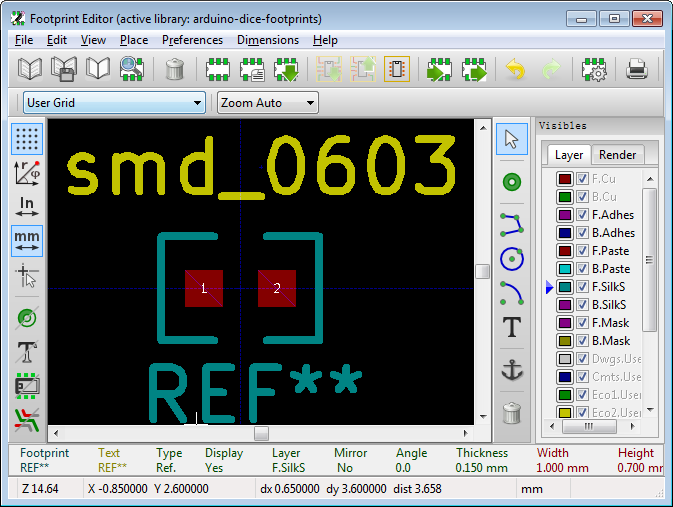
\includegraphics[width=4.5in]{smd_cap_footprint_final}
			\caption{Completed footprint of the SMD 0603 capacitor.}
			\label{fig:smd_cap_footprint_final}
		\end{figure}
			
	\item We wish to create a new library to contain our newly created footprint. To do this, click the ``Create new library and save current module'' icon. Set the location and name of the library and click ``OK''. The ``Library Path'' field should contain the full path to your desired library location. In this example, we will create a footprint library with the name ``arduino-dice-footprints'' (KiCad will automatically add the ``.pretty'' suffix) under the project folder ``...$\backslash$arduino-dice''. Fig.~\ref{fig:create-new-footprint-library} shows the proper settings. At this point, a new folder named ``arduino-dice-footprints.pretty'' should appear in the project tree in the KiCad main window (Fig.~\ref{fig:kicad-footprint-library}). Click on the ``$+$'' sign will expand the library and show all the footprints in this library; in this case, we only have the ``smd\_0603'' footprint.
	
		\begin{figure}[h]
			\centering
			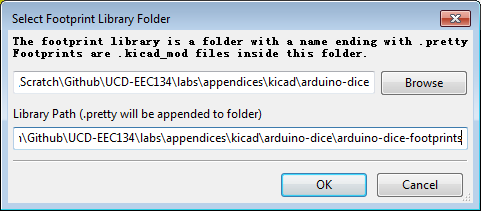
\includegraphics{create-new-footprint-library}
			\caption{The ``Select Footprint Library Folder'' dialog box.}
			\label{fig:create-new-footprint-library}
		\end{figure}

		\begin{figure}[h]
			\centering
			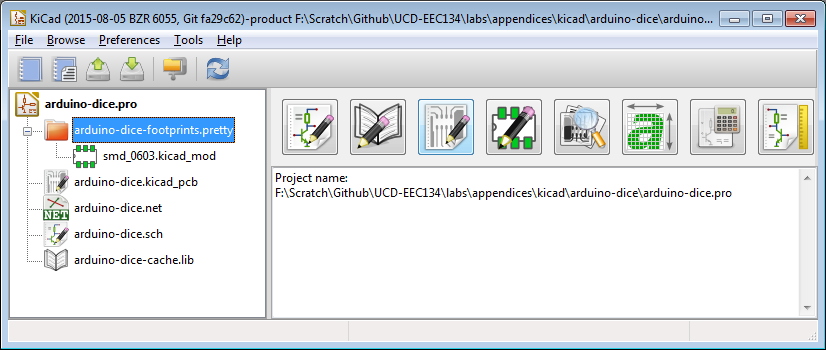
\includegraphics[width=4.5in]{kicad-footprint-library}
			\caption{The new footprint library is now visible in the project tree.}
			\label{fig:kicad-footprint-library}
		\end{figure}
	
	\item Although we now have the new footprint library in our file system and the project tree, KiCad still does not recognize it as part of the available libraries that we can pull footprints from. We will need to manually add the library to KiCad's library tables. 
		\begin{enumerate}
			\item 	Open CvPcb and click the ``Edit footprint library table'' icon. The ``PCB Library Tables'' dialog box should appear. 
			
			\item Click the ``Append with Wizard'' button.
			
			\item In the pop-up dialog box, select ``Files on my computer'' and click ``Next''. 
			
			\item Browse to and select the footprint library folder we just created, click ``Next''. Click ``Next'' again in the next window to confirm. 
			
			\item Select ``To the current project only'' and click ``Finish'' to finish adding the footprint library to this project. If you have created a generic library that you want to use across multiple projects, you could selecte ``To global library configuration'' option. Fig.~\ref{fig:add-project-footprint-lib} shows how the ``PCB Library Tables'' looks like now. Notice how KiCad replaces the absolute path with the ``KIPRJMOD'' variable. 

					\begin{figure}[h]
						\centering
						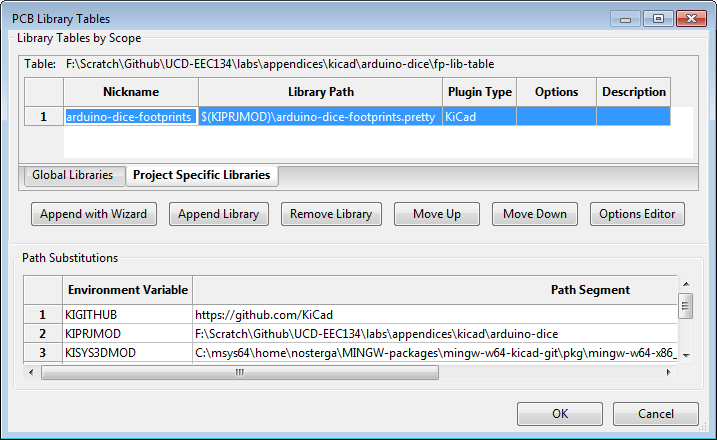
\includegraphics[width=5in]{add-project-footprint-lib}
						\caption{Add a project footprint library.}
						\label{fig:add-project-footprint-lib}
					\end{figure}
		\end{enumerate}

	
\end{enumerate}


\subsection{PCB Layout}




\subsection{Generating Fabrication Files}

\section{Advanced Topics}

\subsection{Controlled Impedance Lines}

* Transmission line parameter calculator: http://wcalc.sourceforge.net/

\section{Further Reading}

* KiCad footprint generator: http://kicad.rohrbacher.net/quickmod.php

* KiCad library management: \url{https://docs.google.com/document/d/1M38ByFyqnhwGo8b_jDDyBceyZtEGeaSAuQaP9REzWrU/edit}


\newpage

\bibliography{pcb}
\bibliographystyle{plain}

\end{document}
